\documentclass[12pt,a4paper]{article}
\usepackage[T1]{fontenc}
\usepackage[polish]{babel}
\usepackage[utf8]{inputenc}
\usepackage{lmodern}
\usepackage{amsmath}
\usepackage{hyperref}
\usepackage{array}
\usepackage{pdflscape}
\usepackage{amsfonts}
\usepackage{graphicx}
\usepackage{longtable}
\usepackage{float}
\selectlanguage{polish}
\usepackage{url}


\usepackage[top=2cm, bottom=2cm, left=3cm, right=3cm]{geometry}
\makeatletter
\newcommand{\linia}{\rule{\linewidth}{0.4mm}}

\newcommand{\Ameryk}{${}^{241}_{}{}$Am }

\renewcommand{\maketitle}{\begin{titlepage}
    \vspace*{1cm}
    \begin{center}\small
    Uniwersytet Warszawski\\
    Wydział Fizyki\\
   Raport z Indywidualnej pracay w laboratorium badawczym
    \end{center}
    
\begin{figure}[h]
    \centering
    
\includegraphics[scale=0.5]{logo.jpg}
    \end{figure}


    \vspace{3cm}
    \noindent\linia
    \begin{center}
      \LARGE \textsc{\@title}
         \end{center}
     \linia
    \vspace{0.5cm}
    \begin{flushright}
    \begin{minipage}{5cm}
    \textit{\small Autor:}\\
    \normalsize \textsc{\@author} \par
    \end{minipage}
    \vspace{5cm}
    
     \end{flushright}
    \vspace*{\stretch{6}}
    \begin{center}
    \@date
    \end{center}
         \end{titlepage}}
    
\makeatother
\author{Filip Kowalski }
\title{Pomiar grubości foli mylarowych przy pomocy promieniowania $\alpha$} 

%pzc
\begin{document}
\maketitle
\begin{abstract}
W czasie ćwiczenia próbowano oszacować grubość foli mylarowych przy pomocy promieniowania $\alpha$. 
\end{abstract}
\section{Wstęp}
Podczas ćwiczenia przygotowano próbki pomiarowe, następnie dokonano kalibracji układu przy pomocy pulsera i źródełka proieniowania $\alpha$. Następnie zmierzono energie cząstek $\alpha$ po przejściu przez próbki mylarowe. Korzystając z danych pomiarowych oraz wyników wygenerowanych przy pomocy programu SRIM, obliczono grubości folii.

\subsection{Kalibracja}
W celu kalibracji układu wykorzystano promieniowanie źródła \Ameryk oraz sygnał generowany przez pulser. Przy wykorzystaniu detektora krzemowego, mierzono kanał promieniowania $\alpha$. Aby móc powiązać kanał z odpowiadającą mu energią cząstki $\alpha$, do kalibracji wykorzystano sygnał z puslera. Zmieniając napięcie  na pulserze, zmierzono zależność kanału od napięcia. Wykres przedstawiający zmierzone wartości przedstawiono na rysunku \ref{kalibracja}. Znając napięcie oraz numer kanału (uzyskane wartości umieszczono w tablicy [DODAĆ TABLICE]. Znając energię $\alpha$ emitowaną przez \Ameryk  (5.486 MeV) dopasowano ....

\subsection{Pomiar}






\begin{figure}[H]
\centering
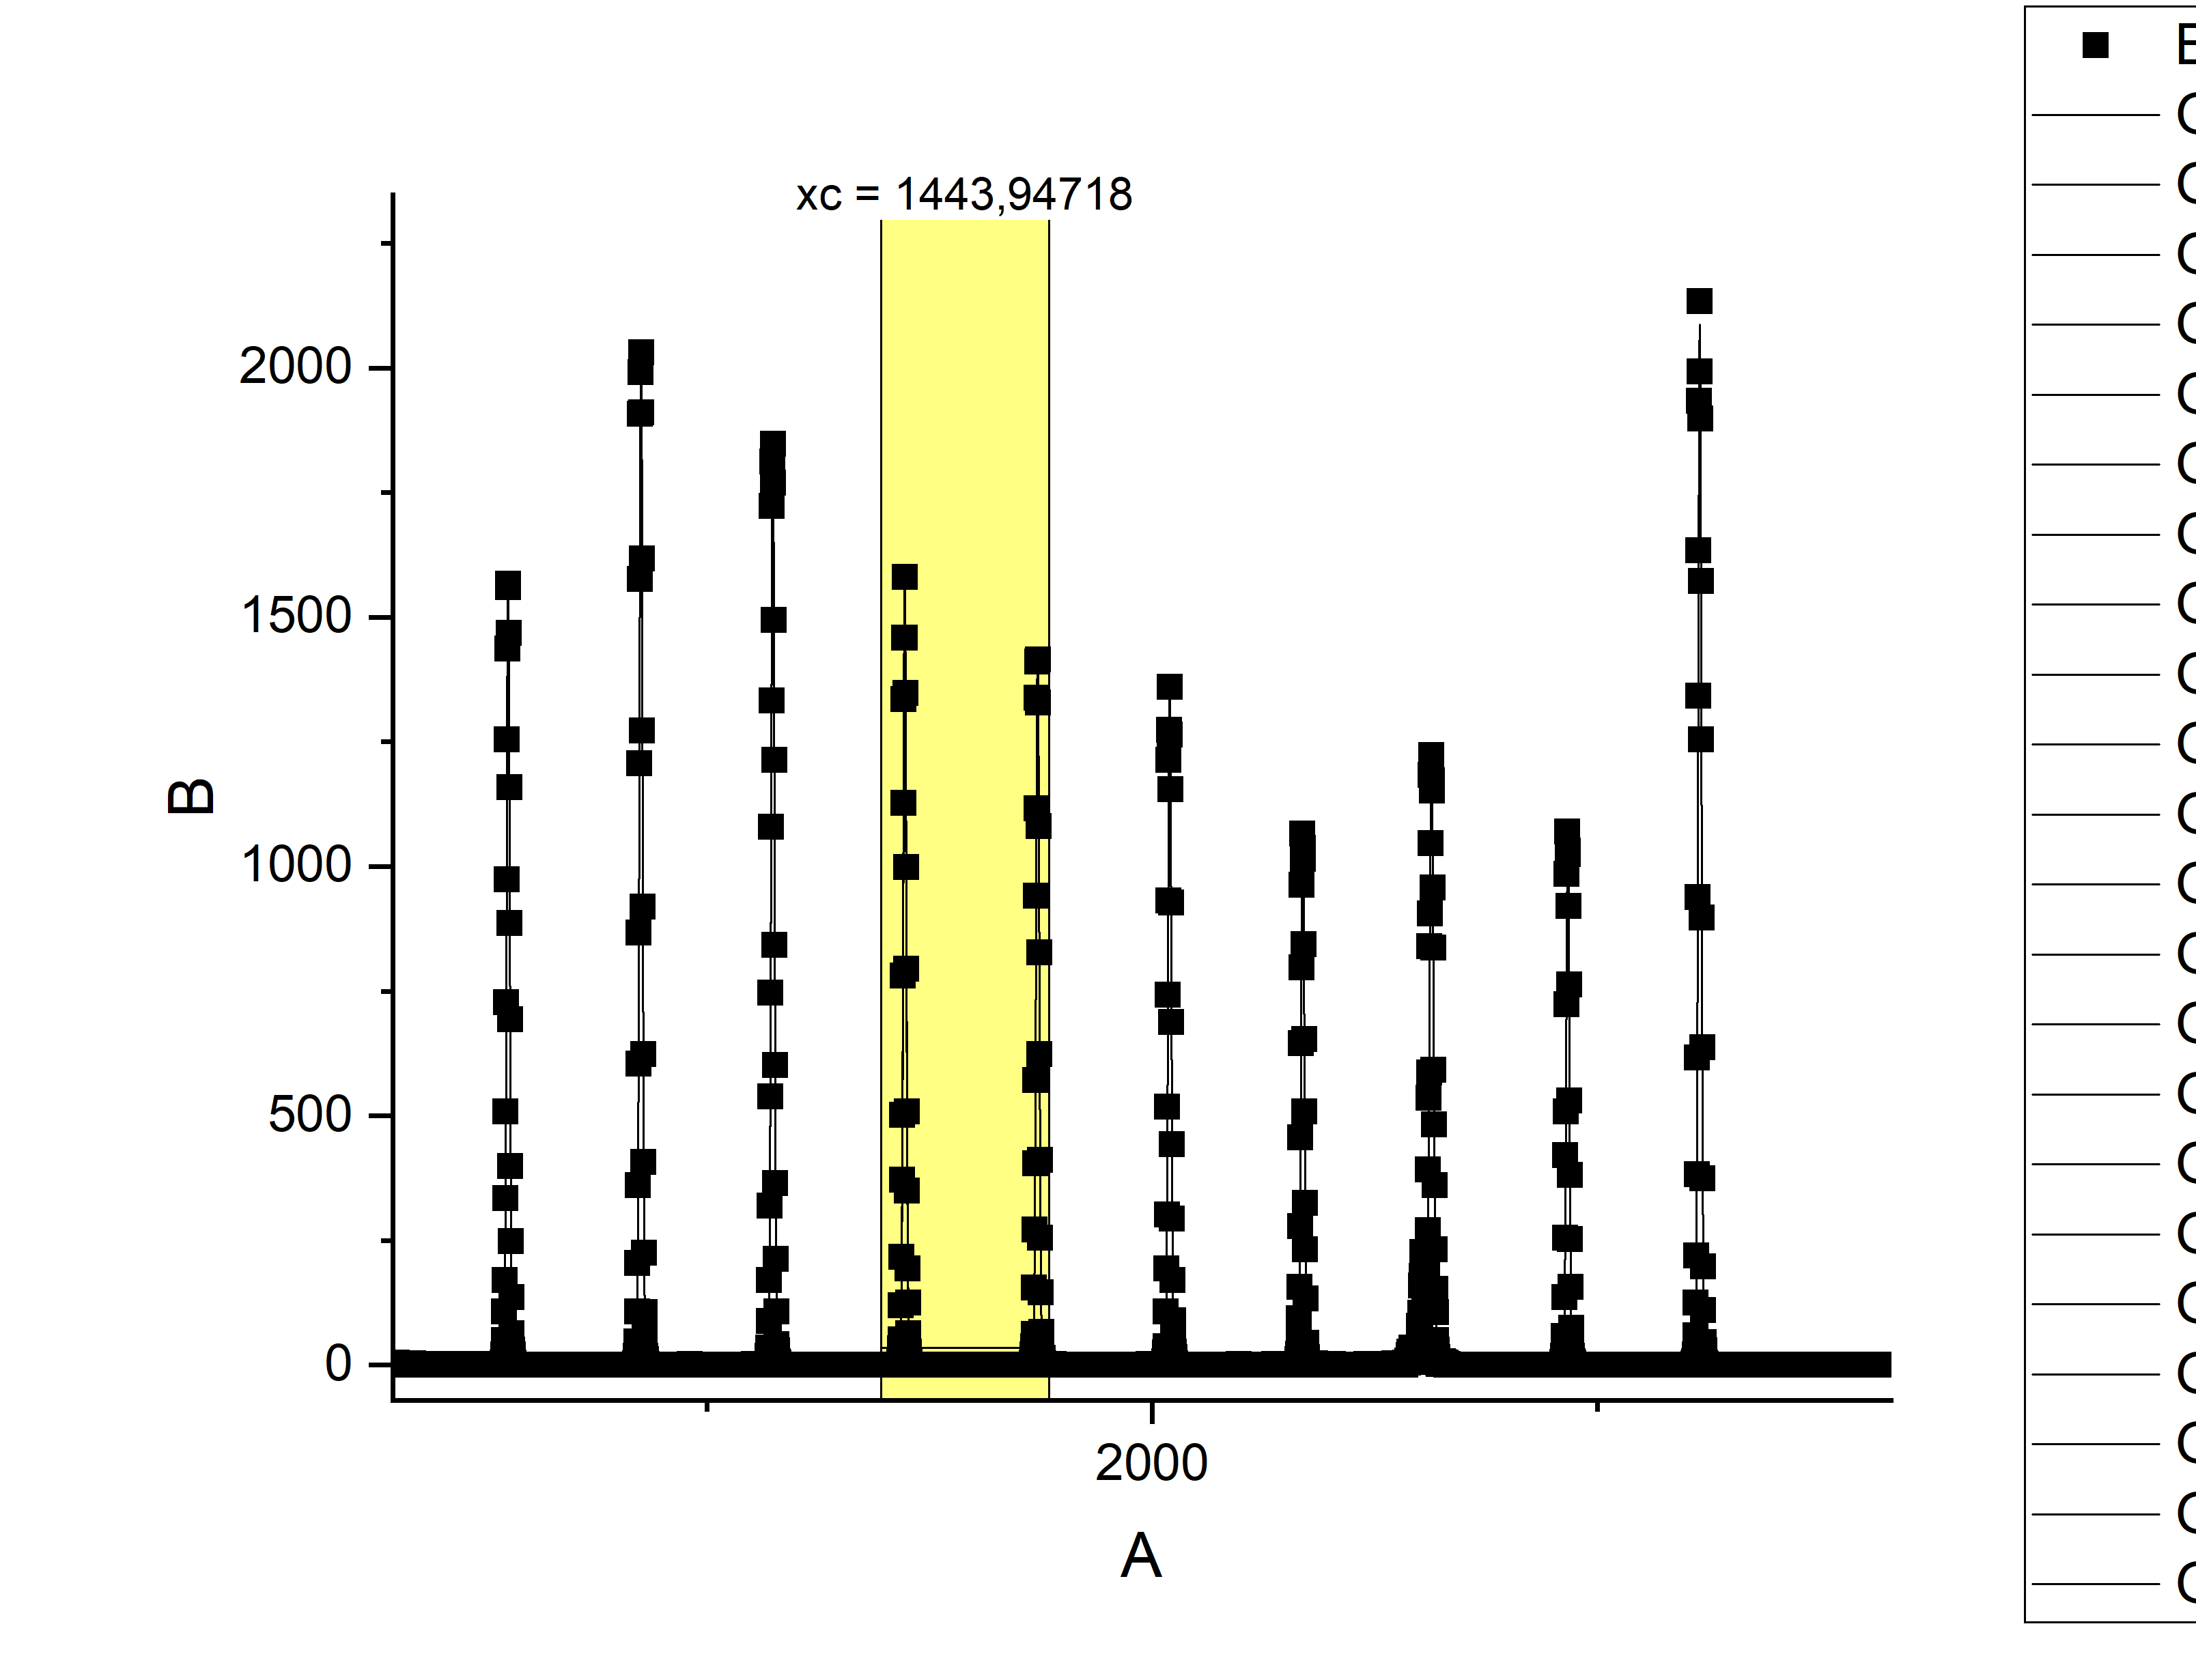
\includegraphics[scale=0.5]{kalibracja.png}
\caption{Zliczenia w zależności od kanału - pomiar kalibracyjny}
\label{kalibracja}
\end{figure}



\subsection{Metoda pomiaru}


\section{Prezentacja wyników}

\begin{figure}[H]
\centering

\includegraphics[scale=.6]{obrazek.jpg}
\caption{Wykres}
\label{moc od oporu}
\end{figure}













\section{Dyskusja wyników i obserwacja}
Dyskusja 

\begin{thebibliography}{9}
\bibitem{ins} 
Instrukcja do ćwiczenia
\url{http://psi.fuw.edu.pl/bin/view/IPWb/PojemnoscCieplnaZarowki}
\end{thebibliography}
\end{document}
